\chapter{DISPATCH OPTIMIZATION STRATEGIES AND SIMULATION EXPERIMENTS}

\section{The Municipal Resource Allocation Dilemma}
In municipal public works management, desilting and drain clearance operations are constrained by finite municipal resources. A municipal corporation such as CMC typically operates with a limited fleet of suction desilting tankers, mechanical backhoes, and manual maintenance crews. Under standard pre-monsoon or emergency storm conditions, municipal crews can only intervene upon a modest budget of $K$ conduits (where $K$ typically ranges between 10 and 500 segments across a city containing nearly 14,000 conduits).

The fundamental municipal optimization question is: \textit{Given a strict budget of $K$ conduit interventions and an impending storm of intensity $i$, which specific conduits should be cleared to maximize systemic flood risk reduction across the entire urban network?}

Historically, municipal engineers prioritize conduits exhibiting the highest visible blockage or sediment percentage. However, in a directed hydraulic network, isolated severity does not equate to systemic impact. A completely clogged headwater ditch with zero upstream tributaries impacts only its immediate road shoulder. In contrast, clearing a moderately or severely clogged downstream trunk line that serves as the primary outflow bottleneck for dozens of upstream residential wards relieves hydraulic backwater pressure across the entire tributary basin.

\section{Proposed Cascade-Aware Dispatch Strategy}
CivicTwin introduces a multi-criteria, lexicographical ranking strategy termed \textbf{Cascade-Aware Prioritization}. The algorithm evaluates all candidate conduits $v \in V_{\text{cand}}$ that are currently \texttt{OPEN} and georeferenced within municipal corporation limits. 

The strategy establishes a strict hierarchical sort key:
\begin{equation}
\text{Key}_{\text{cascade}}(v) = \Big(-T(v, i),~ -C_{\text{saved}}(v),~ -U(v, i),~ v\Big)
\label{eqn:cascade_sort_key}
\end{equation}
where:
\begin{enumerate}
    \item \textbf{Primary Criterion: Categorical Threat Tier ($-T(v, i)$):} Conduits are prioritized first by hydraulic failure urgency. All Critical conduits ($T = 2$, utilization $> 125\%$, active overflow) must be scheduled before High threat conduits ($T = 1$), which in turn precede Low threat conduits ($T = 0$).
    \item \textbf{Secondary Criterion: Upstream Cascade Reachability ($-C_{\text{saved}}(v)$):} Within a given threat tier, conduits are ranked by the cardinality of their upstream ancestor set $|\text{anc}(v)|$. A critical conduit whose clearance relieves 1,300 upstream conduits is dispatched before a critical conduit that relieves only 20 upstream conduits.
    \item \textbf{Tertiary Criterion: Local Capacity Utilisation ($-U(v, i)$):} For conduits tied in both threat tier and cascade reachability, priority is assigned to the conduit carrying the highest local surcharge ratio $U(v, i)$.
    \item \textbf{Deterministic Tie-Breaker ($v$):} Stable tie-breaking is enforced using unique internal segment indices.
\end{enumerate}

By structuring the prioritization hierarchically, the cascade-aware strategy targets acute emergency bottlenecks while maximizing systemic network relief.

\section{Comparative Baseline Strategies and Ablation Formulations}
To rigorously benchmark the proposed cascade-aware strategy, CivicTwin implements three comparative strategies:
\begin{enumerate}
    \item \textbf{Local Severity-Only (Standard Municipal Baseline):}
    Emulates prevailing municipal practice by prioritizing conduits purely according to local capacity exhaustion:
    \begin{equation}
    \text{Key}_{\text{severity}}(v) = \Big(-U(v, i),~ -C_{\text{saved}}(v),~ v\Big)
    \label{eqn:severity_sort_key}
    \end{equation}
    This heuristic clears the most overloaded channels regardless of whether they are situated at isolated headwaters or arterial trunk lines.
    \item \textbf{Cascade-Only (Ablation Baseline):}
    Ranks conduits purely by upstream reachability without regard to immediate threat tier:
    \begin{equation}
    \text{Key}_{\text{cascade\_only}}(v) = \Big(-C_{\text{saved}}(v),~ -U(v, i),~ v\Big)
    \label{eqn:cascade_only_key}
    \end{equation}
    This ablation evaluates whether topological connectivity alone is sufficient for optimal dispatch, or whether the hierarchical combination of threat tier and reachability is essential.
    \item \textbf{Random Dispatch (Stochastic Baseline):}
    Selects candidate conduits uniformly at random:
    \begin{equation}
    \pi_{\text{random}} \sim \text{UniformPermutation}(V_{\text{cand}})
    \end{equation}
    To eliminate stochastic bias, the random baseline is evaluated across 20 distinct random pseudo-random seeds ($S = 20$), reporting sample means and standard deviations.
\end{enumerate}

\section{Closed-Loop Simulation Lifecycle and Feedback Dynamics}
In operational deployment and experimental simulations, conduit dispatch follows a formal three-state finite state machine, as depicted in Figure~\ref{fig:fsm_lifecycle}.

\begin{figure}[h!]
\centering
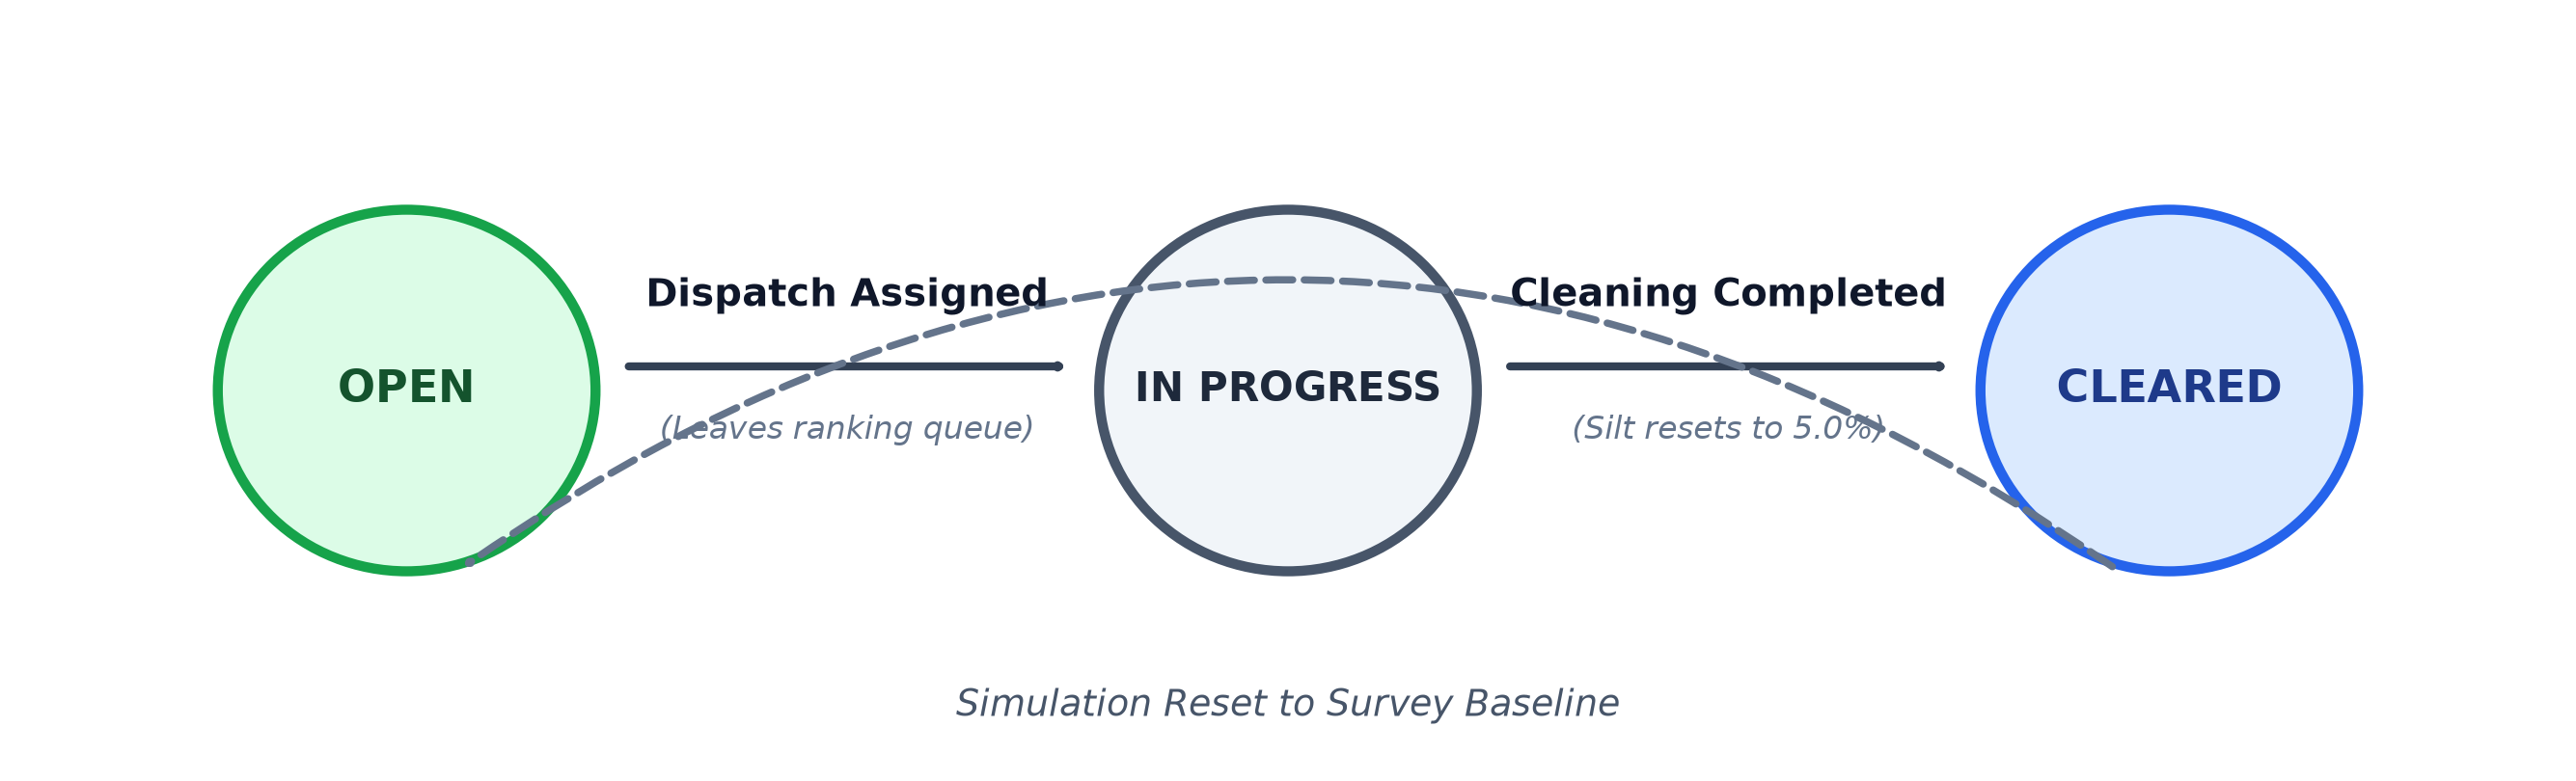
\includegraphics[width=0.85\textwidth]{figures/fig_fsm_lifecycle.png}
\caption{Conduit Operational State Lifecycle in CivicTwin}
\label{fig:fsm_lifecycle}
\end{figure}

The state transition mechanics are formalized as follows:
\begin{itemize}
    \item \textbf{\texttt{OPEN} State ($S = 0$):} Conduit is unassigned and subject to active ranking under the chosen strategy.
    \item \textbf{\texttt{IN\_PROGRESS} State ($S = 1$):} Upon dispatch by an operator, the conduit is assigned to an active field work crew. It is immediately removed from the top-$k$ candidate ranking and transferred to the active dispatch queue. This dynamic backfilling moves the next highest-ranked conduit into the top-$k$ view without human latency.
    \item \textbf{\texttt{CLEARED} State ($S = 2$):} When the field crew logs completion, the conduit's silt buildup resets to the post-cleaning baseline:
    \begin{equation}
    S(v) \leftarrow S_{\text{clean}} = 5.0\%
    \end{equation}
    The effective capacity $Q_{\text{avail}}(v)$ expands to 95\% of design capacity (Eqn.~\ref{eqn:avail_capacity}). The engine instantly recalculates network risk exposure $E_{\text{net}}$, logging the exact exposure delta $(\Delta E_{\text{net}} = E_{\text{net}}^{\text{before}} - E_{\text{net}}^{\text{after}})$ to the audit trail.
\end{itemize}

\section{Simulation Experimental Design}
To evaluate the relative efficacy of the dispatch strategies, an automated Monte Carlo experiment script (\texttt{run\_experiment.py}) was executed against the complete 13,998 conduit network. 

The experimental matrix spans:
\begin{itemize}
    \item \textbf{Precipitation Intensities ($i$):} 80~mm/hr (heavy monsoon rain), 120~mm/hr (severe monsoon cloudburst), and 160~mm/hr (extreme convective deluge).
    \item \textbf{Clearing Budgets ($K$):} Evaluated at steps $K \in \{10, 50, 100, 250, 500\}$ completed desilting actions.
    \item \textbf{Evaluation Metrics:}
    \begin{enumerate}
        \item \textbf{Exposure Reduction Percentage ($\Delta E_{\text{net}}\%$):} The percentage reduction in systemic network risk exposure from baseline:
        \begin{equation}
        \Delta E_{\text{net}}\% = \frac{E_{\text{net}}^{(0)} - E_{\text{net}}^{(K)}}{E_{\text{net}}^{(0)}} \times 100
        \end{equation}
        \item \textbf{At-Risk Drains Resolved:} Conduits whose own capacity utilization or whose downstream bottleneck utilization is reduced below 100\%, eliminating active overflow and backwater surcharge risks.
        \item \textbf{Over-Capacity Drains Resolved:} Conduits whose individual flow exceeds 100\% capacity that are directly returned to safe flow levels ($U \le 1.0$).
        \item \textbf{Critical Drains Resolved:} Conduits whose utilization is reduced from Critical ($> 125\%$) to safe levels.
        \item \textbf{Distinct Drains Relieved:} Total number of distinct conduits lying upstream of or comprising the cleared segments ($\bigcup_{k=1}^K (\text{anc}(v_k) \cup \{v_k\})$).
    \end{enumerate}
\end{itemize}
All strategies were initialized from identical baseline survey conditions to ensure rigorous comparative equity.
